\documentclass{report}


%%%%%%%%%%%%%%%%%%
%   Liste des packages utilisés  %
%%%%%%%%%%%%%%%%%%

% (oui y'en a 95% qui sont inutiles ^^)

\usepackage{amssymb}
\usepackage{array}
\usepackage{hyperref}
\usepackage{booktabs}
\usepackage{multirow}
\usepackage{float}
\usepackage{lmodern} %Pack de police
\usepackage{color}
\usepackage[dvipsnames]{xcolor}
\usepackage{graphicx}
\usepackage[utf8x]{inputenc}
\usepackage[T1]{fontenc}
\usepackage{natbib}
\usepackage[francais]{babel}
\usepackage{caption}
\usepackage{listings}
\usepackage{booktabs}
\usepackage[top=2cm, bottom=2cm,left=2cm, right=2cm]{geometry}
\usepackage{blindtext}
\usepackage{setspace}
\usepackage{graphicx}
\usepackage{titlesec, blindtext, color} % titres spéciaux + couleur pour les chapter

% on transforme les chapters en juste le numéro suivi du titre, avec un barre grisse
\definecolor{gray75}{gray}{0.75}
\newcommand{\hsp}{\hspace{20pt}}
\titleformat{\chapter}[hang]{\Huge\bfseries}{\thechapter\hsp\textcolor{gray75}{|}\hsp}{0pt}{\Huge\bfseries}

\begin{document}


%%%%%%%%%%%
%  Page de garde  %
%%%%%%%%%%%
\begin{titlepage}
	\begin{center}
	
		\begin{spacing}{1.5}
			Projet Picross\\
			\vspace*{\fill}
		\end{spacing}
		
		\begin{spacing}{2.5}
			\textbf{\Huge Application de création et d'aide à la résolution de puzzle \textit{picross}}\\[0.5cm]
			\textbf{\huge Cahier des charges} \\
			\vspace*{\fill}
			\textit{Étudiants :}
		\end{spacing}

		\begin{spacing}{1.15}
			\large
			\textsc{Brinon} Baptiste\\
			\textsc{Brocherieux} Thibault\\
			\textsc{Cohen} Mehdi\\
			\textsc{Debonne} Valentin\\
			\textsc{Lardy} Anthony\\
			\textsc{Mottier} Emeric\\
			\textsc{Pastouret} Gilles\\
			\textsc{Pelloin} Valentin\\
			\vspace*{\fill}
			\textbf{Groupe n\up{o}2} \\
			\textnormal{\large Licence Informatique\\ Le Mans Université\\ \today}
		\end{spacing}
		
	\end{center}
\end{titlepage}


%%%%%%%%%%
%    Sommaire    %
%%%%%%%%%%
\renewcommand{\contentsname}{Sommaire}
\tableofcontents


\chapter{Présentation}

	\section{Introduction}

		Dans le cadre de l'unité d'enseignement « Génie logiciel 2 » de la Licence d'informatique de Le Mans Université, les étudiants de troisième année sont amenés à travailler sur un projet de développement d'une application. \\
		Ce document décrit le contexte, les besoins fonctionnels, les objectifs et les contraintes définis par les clients. Un premier découpage des étapes nécessaires à la réalisation du projet donne lieu dans le document à un planning prévisionnel.

	
 	\section{Objectif de l'application}		
		Nous devons réaliser un jeu de type picross (aussi appelé \textit{nonogramme}, logigramme ou \textit{hanjie}) permettant à un utilisateur de résoudre des grilles et de l'aider dans sa réalisation.

	\section{Règles du \textit{picross}}
		Le picross est un jeu de type puzzle. Le jeu consiste à découvrir un dessin sur une grille en noircissant des cases d'après des indices donnés.	
		Pour pouvoir déterminer les cases à colorier, on dispose de groupes de nombres indiqués à une extrémité de chaque ligne et colonne.
		\newline
		Les nombres indiqués permettent d'identifier la taille des blocs de cases à colorier sur la ligne ou colonne ainsi que leur ordre.
		\newline
		Chaque groupe de cases doit être séparé des autres par une case blanche ou plus.
	
		
\chapter{Spécification des besoins}

		\section{Mode de jeu}
			Le jeu est composé de plusieurs chapitres de plus en plus difficiles. Chaque chapitre regroupe des grilles de différentes tailles. Au début du jeu, seul le premier chapitre est débloqué et les autres se débloquent au fur et à mesure que le joueur termine les grilles.\\
			Un chapitre à part du mode de jeu classique contient des niveaux particuliers où la grille évolue durant la partie. Dans ces niveaux, la taille de la grille augmente à mesure que l'utilisateur complète la grille existante.

		\section{Score}
			On évalue le score d'un joueur sur une grille par le nombre d'étoiles obtenues. Un joueur peut gagner quatre étoiles par grille au maximum. Le nombre d'étoiles décernées au joueur lorsque celui-ci termine le niveau est calculé en fonction du temps qu'il a mis à résoudre la grille. Chaque chapitre du jeu se débloque automatiquement dès que le nombre d'étoiles requis à son déverrouillage est atteint. Plus un chapitre contient de grilles difficiles, plus le nombre d'étoiles requises est élevé.\\
			Durant une partie, le joueur peut mettre le jeu en pause à n'importe quel moment, le chronomètre est alors mis en pause.

				
		\section{Statistiques}
			En plus du score, l'application garde en mémoire certaines statistiques associées au joueur ainsi qu'aux grilles. Les statistiques du joueur comportent son score total (nombre total d'étoiles), le nombre de niveaux et de chapitres réussis. Les statistiques pour chaque grille sont le meilleur temps effectué par le joueur, le nombre d'aides utilisées ainsi que le nombre d'erreurs effectuées lors de ce meilleur temps.

			
		\section{Aide}
			Plusieurs aides sont proposées aux joueurs. Le type d'aide dépend de la difficulté du chapitre. Pour un chapitre facile, l'aide colorie directement une case correcte sur la grille. Pour un chapitre de difficulté moyenne, l'aide indique la ligne ou la colonne où se trouve une case correcte non coloriée. Pour un chapitre difficile, l'aide indique si le joueur a colorié une case incorrecte. Plus le joueur avance dans des chapitres difficiles, moins celui-ci est autorisé à utiliser d'aides au cours de sa partie de \textit{picross}.

		\section{Hypothèses}			
			À tout moment durant une partie, le joueur peut décider d'utiliser le mode hypothèse. Durant celui-ci, les cases qu'il remplit par la suite sont d'une autre couleur que celle de base. Il peut créer jusqu'à cinq hypothèses simultanées, imbriquées les unes dans les autres.\\
			Si le joueur se rend compte que l'une de ses hypothèses est fausse, il peut l'annuler. Cela a pour effet de supprimer toutes les autres hypothèses posées après celle annulée. Ceci le fait donc revenir à l'état de l'hypothèse précédente.\\
			En revanche, il peut décider qu'une hypothèse est vraie. Dans ce cas, toutes les autres hypothèses qui interviennent avant celle-ci le deviennent aussi. Les cases colorées changent alors de couleur, et deviennent des cases normales.
		
		\section{Didacticiel}
			Un chapitre de l'application est présent comme didacticiel. Ce chapitre est optionnel et permet aux joueurs débutants de se familiariser avec les règles du \textit{picross}. Il consiste en plusieurs parties guidées d'une grille simple de \textit{picross} en expliquant au joueur les actions à réaliser étape par étape afin de finir la grille. L'application contient également un rappel des règles générales du \textit{picross}.
			
		\section{Interface homme-machine}
			L'application est utilisable intégralement à la souris ou au clavier ou en utilisant les deux, au choix de l'utilisateur.\\
			L'utilisateur peut également sélectionner une suite de cases verticale ou horizontale et de la colorier d'un seul coup, à la souris comme au clavier. Lors de cette sélection, le nombre de cases sélectionnées est affiché.\\
			L'application sauvegarde automatiquement la partie après chaque action du joueur afin de pouvoir reprendre n'importe quelle grille à n'importe quel moment.
			L'application est disponible en français et en anglais, avec un système qui permet de rajouter des langues supplémentaires ultérieurement.
			
\chapter{Spécification des contraintes}

	\section{Conception}
		Le client demande que le logiciel soit réalisé en Ruby, et que la documentation soit engendrée via \textit{RDoc}. Celle-ci sera livrée avec les livrables. L'interface doit être programmée avec \textit{GTK}.
		
	\section{Cartes et interface}
		Une carte doit être seulement en noir et blanc afin de ne pas confondre des cases colorées avec les hypothèses qui sont elles aussi colorées.
		La grille doit prendre suffisamment de place sur la fenêtre de manière à être facilement lisible malgré l'importante quantité de chiffres et l'interface, et ce, qu'importe la taille de la fenêtre. En lien avec cela, la taille de grille n'excède pas 25 par 25.
		Lorsqu'une carte est complète, elle doit représenter une forme évocatrice en noir et blanc.
	
	\section{Limitation de l'aide}
		L'utilisation de l'aide n'a pas de limite. Pour éviter cela, une pénalité est appliquée lors de l'utilisation de celle-ci. Une perte de temps est infligée lors de l'utilisation d'une aide. Ceci peut donc impacter les étoiles remportées à la fin de la partie. La pénalité et le temps de jeu sont indiqués séparément. Le total est pris en compte au moment du calcul du score. De plus le joueur possède des aides n'infligeant pas de pénalité. Celles-ci sont obtenues lorsque le joueur complète des niveaux. 
	
	\section{\textit{Gameplay}}
		Lors d'une pause, le chronomètre est arrêté. Le joueur pourrait ainsi résoudre le \textit{picross} sans que le temps ne défile, ce qui briserait le système de scores. Pour éviter cela, on effectue un masquage de la grille.
		
	\section{Didacticiel}
		Le didacticiel est jouable à n'importe quel moment. Il se trouve dans un chapitre spécial. Ce chapitre n'est pas obligatoire. Ce chapitre octroie tout de même des étoiles. \\
		Il contient le nécessaire pour expliquer toutes les règles ainsi que le fonctionnement du logiciel (explication de l'interface, système de score).
	
	\section{Sauvegardes \& hypothèses}
		Les sauvegardes sont réalisées automatiquement. L'utilisateur ne peut donc pas réaliser de sauvegardes manuelles. Lors d'une sauvegarde, l'ensemble des hypothèses de la partie sont enregistrées distinctement. Le nombre d'hypothèses est limité afin de conserver la clarté de la carte. Le maximum est fixé à 5 hypothèses simultanées.
	
	\section{Délais}
		Le programme doit être terminé pour le 12 avril 2018, soit approximativement 3 mois pour réaliser le projet. L'utilisation de ce temps est indiquée sur le diagramme de \textit{Gantt} suivant :

	\begin{figure}[H]
		\centering
		\caption{Diagramme de \textit{Gantt} général du projet}
		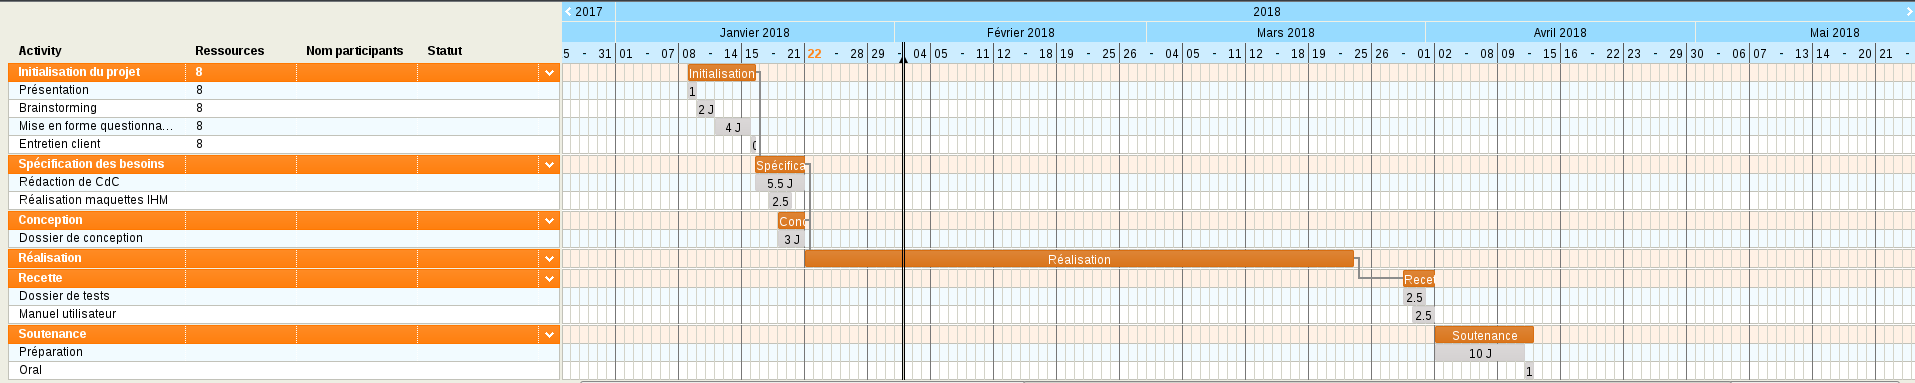
\includegraphics[width=17cm]{ganttGeneral.png}
	\end{figure}	     
		
		
\chapter{Livrables attendus}
	Les livrables rendus à l'issue de ce projet sont :
	\begin{itemize}
	\item Le cahier des charges
	\item Le cahier de conception
	\item Le logiciel terminé et fonctionnel
	\item La documentation (\textit{RDoc})
	\item Le manuel utilisateur
	\end{itemize}
		
%	``I always thought something was fundamentally wrong with the universe'' \citep{adams1995hitchhiker}	
		\bibliographystyle{plain}
		\bibliography{references}

\end{document}
